\documentclass{scrartcl}

\usepackage[utf8]{inputenc}
\usepackage[T1]{fontenc}
\usepackage[english]{babel}

\usepackage{enumerate}
\usepackage{hyperref}
\usepackage{caption}
\usepackage{subcaption}

% Math 
\usepackage{amsmath}
\usepackage{amssymb}
\usepackage{amsthm}
\usepackage{mathtools}
\usepackage{dsfont}
\usepackage{BOONDOX-calo}
\usepackage{stmaryrd}


% Graphics
\usepackage{graphicx}
\usepackage{svg}
\usepackage{tikz}
\usepackage{tikz-cd}
\usetikzlibrary{trees}
\usetikzlibrary{cd}


\theoremstyle{plain}
\newtheorem{theorem}{Theorem}[section]
\newtheorem{theorem*}{Theorem}
\newtheorem{proposition}[theorem]{Proposition}
\newtheorem{proposition*}[theorem*]{Proposition}
\newtheorem{corollary}[theorem]{Corollary}
\newtheorem{lemma}[theorem]{Lemma}
\newtheorem{conjecture}[theorem]{Conjecture}

\theoremstyle{definition}
\newtheorem{definition}[theorem]{Definition}
\newtheorem{definition*}[theorem*]{Definition}
\newtheorem{example}[theorem]{Example}
\newtheorem{examples}[theorem]{Examples}
\newtheorem{remark}[theorem]{Remark}
\newtheorem{remarks}[theorem]{Remarks}
\newtheorem{warning}[theorem]{Warning}
\newtheorem{hypothesis}[theorem]{Hypothesis}
\newtheorem{hypothesis*}[theorem*]{Hypothesis}
\newtheorem{construction}[theorem]{Construction}


\newcommand{\A}{\mathbb A}
\newcommand{\C}{\mathbb C}
\newcommand{\N}{\mathbb N}
\newcommand{\R}{\mathbb R}
\newcommand{\Q}{\mathbb Q}
\newcommand{\Z}{\mathbb Z}

\renewcommand{\emptyset}{\varnothing}
\renewcommand{\epsilon}{\varepsilon}
\renewcommand{\subset}{\subseteq}
\renewcommand{\supset}{\supseteq}

\newcommand{\hteq}{\simeq}
\newcommand{\iso}{\cong}
\newcommand{\defeq}{\coloneqq}
\newcommand{\from}{\leftarrow}

\DeclareMathOperator{\Hom}{Hom}
\DeclareMathOperator{\holim}{holim}
%\DeclareMathOperator{\lim}{lim}
\DeclareMathOperator{\hocolim}{hocolim}
\DeclareMathOperator{\colim}{colim}

\DeclareMathOperator{\Conf}{Conf}
\DeclareMathOperator{\UConf}{Conf}
\DeclareMathOperator{\cConf}{\overline{Conf}}

\DeclareMathOperator{\coGra}{{}^*Gra}
\DeclareMathOperator{\Gra}{Gra}
\DeclareMathOperator{\coGraphs}{{}^*Graphs}
\DeclareMathOperator{\Graphs}{Graphs}

%\newcommand{\Coprod}{\coprod}
\renewcommand{\coprod}{\amalg}
\newcommand{\Prod}{\prod}

\newcommand{\realization}[1]{\left\lvert#1\right\rvert}
\newcommand{\totalization}[1]{\left\lVert#1\right\rVert}

\newcommand{\abs}[1]{\left\lvert#1\right\rvert}
\newcommand{\norm}[1]{\left\lVert#1\right\rVert}

\newcommand{\iHom}{\underline{\operatorname{Hom}}}

\newcommand{\blank}{-}
\newcommand{\comp}{\circ}

\newcommand{\grVec}{\mathrm{gr{-}Vec}}

% Bibliography
\bibliographystyle{alpha}


\begin{document}
\section{Pullback-Pushout Lemma}
Consider the following pullback of topological spaces:
\begin{center}
\begin{tikzcd}
    E\times_B X \arrow[d] \arrow[r] & E \arrow[d]{p} \\
    X \arrow[r] & B
\end{tikzcd}
\end{center}

We are interested in describing the chain complex of $E\times_B X$ using the chain complexes of the span $X \to B \leftarrow E$. Since homology is a homotopy invariant, it makes sense to consider this as a homotopy pullback; this is the case for example if the vertical arrows are fibrations. The general statement that one might hope for here is that the homotopy pullback commutes with the chain complex functor. This is wrong in general, however it is true under certain connectedness assumptions on the involved spaces. 

We first state the version of the statement from~\cite{felix2012rational}
\begin{theorem}
Assume $p$ is a Serre fibration, $E$ is path connected and $X$ and $B$ are simply connected. Let $A_X \leftarrow A_B \rightarrow A_E$ be a rational dgca model for the lower right zigzag in the diagram. Then the homotopy pushout $A_X \otimes_{A_B}^h A_E$ is a dgca model for the pullback $E\times_B X$.  
\end{theorem}
For the proof they reference~\cite[Proposition 15.8]{naef2022string}, where this is shown in the case that $A_X$, $A_E$ and $A_B$ are Sullivan models. By homotopy invariance of the homotopy pushout, this then also holds for dgca models. Note that field coefficients are used here. 

Homotopy limits take a bit of time to describe and we do not go in-depth here. The basic problem is that homotopy equivalent diagrams of e.g.\ spaces or chain complexes generally don't yield homotopy equivalent limits resp.\ colimits. One also cannot work in the homotopy category, where homotopic maps are identified, as this category is known to not have many limits resp.\ colimits. 

There are two basic ideas to computing homotopy limits. The first is to replace the diagram with a homotopy equivalent version that is somehow general enough that the usual limit construction gives the correct homotopy pushout. An investigation of the properties that make this work leads to the notion of model categories, which are categories equipped with distinguished classes of morphisms, namely weak equivalences, cofibrations and fibrations. See for example~\cite{dwyer1995homotopy} (TODO other references).

The second idea is to make homotopies between maps, and higher homotopies part of the structure of the category, which leads to the notion of $\infty$-categories~\cite{lurie2009higher},\ \cite{lurie2017higher} (TODO other references) (also known as quasicategories or $(\infty, 1)$-categories). In an $\infty$-category, composition of morphisms is only defined up to homotopy. Much of the language and theorems of regular categories translate to $\infty$-categories. A notion of limits and colimits in $\infty$-categories exists and it agrees with homotopy limits resp.~colimits in the examples. We briefly unpack what this means for pullbacks. Recall that in a normal pullback, to every cone, the pullback assigns a universal arrow to the pullback cone, which makes certain triangles commute. In homotopy, these triangles commute only up to homotopy and we consider homotopies part of the data. Hence a cone consists not only of natural morphisms, but also of explicit homotopies that make the relevant triangles commute up to homotopy. The pullback is a universal cone and the universal property assigns to each cone not only a universal arrow, but also homotopies which make the relevant diagrams commute. As this assignment depends on the cone, it depends not only on the morphisms of the cone, but also on the homotopies. This assignment is no longer unique, instead one requires that the space of suitable data is contractible, which is where higher homotopies appear. 

There is a homology version of the theorem, this is the Eilenberg-Moore spectral sequence~\cite{eilenberg1966homology}. 

Note that there is an equivalent pullback diagram
\begin{center}
\begin{tikzcd}
    E\times_B X \arrow[d] \arrow[r] & B \arrow[d] \\
    E\times X \arrow[r] & B \times B
\end{tikzcd}
\end{center}
which identifies the homotopy fiber of the vertical maps, hence there is a homotopy fiber sequence $\Omega B \to E\times_B X \to E\times X$, i.e. the homotopy fiber of $E\times_B X \to E\times X$ is the loop space $\Omega B$.


\section{Configuration Spaces}

\paragraph{Definition} For $X$ a topological space resp.\ a set, let
\begin{align*}
    \Conf_X(n) = \{(x_1,\dots, x_n)\in X^n \mid x_i \neq x_j\ \text{if}\ i\neq j\}
\end{align*}
We write $\Conf_m(n) \coloneqq \Conf_{\R^m(n)}$. Note for a natural number $n$, we write $\underline n \defeq \{1, \dots, n\}$; thus we can write $\Conf_{\underline m}(n)$, which is a finite set and not a space. 

\paragraph{Homotopy Properties} The configuration spaces are homotopy equivalent to the little disks operad. For an overview of properties of the little disks operad see~\cite{fresse2017homotopy}. There is a recognition principle by Fiedorowicz, which gives sufficient conditions for an operad to be homotopy equivalent to the little 2-disks operad. There is no higher-dimensional analogue, because the recognition principle relies on the universal covering. 

\paragraph{Fadell-Neuwirth Tower} There is a tower of fibrations $\Conf_m(n) \to \Conf_m(n-1) \to \dots \to \Conf_m(2) \simeq S^{m-1}$, which split (e.g. by adding a point at infinity or duplicating the $i$th point). The fiber sequence is $\bigvee_{n-1} S^{m-1} \to \Conf_m(n) \to \Conf_m(n-1)$. Check Lem 3.4 in~\cite{sinha2010homology}. 

\subsection{Homology and Cohomology} 
It is well-known that $H^*(\Conf_m(n))$ is the free graded commutative algebra generated by $\alpha_{ij}$ with degree $1$ modulo the relations $\alpha_{ij} = \pm\alpha_{ji}$, $\alpha_{ii}=0$ and $\alpha_{ij}\alpha_{jk} + \alpha_{jk}\alpha_{ki} + \alpha_{ki}\alpha_{ij} = 0$. The generators are given by $\pi_{ij}^*\omega$ for $\omega\in C^{m-1}(\Conf_m(2))$ representing a fundamental cohomology class, (note the homotopy equivalence $\Conf_m(2)\simeq S^{m-1}$). This is a classical result by Arnol'd, proven via spectral sequences, through analysis of the fibration maps $\Conf_m(n) \to \Conf_m(n-1)$. 

In homology, it is known that $H_*(\Conf_m(n))$ is the Gerstenhaber operad for $m=2$ and an analog for $m>2$. Explicitly, this is the universal operad generated by $\mu\in H_0(\Conf_m(2))$ and $b\in H_{m-1}(2)$, where $\mu$ is commutative and associative, $b$ is anticommutative and satisfies the Jacobi identity, and both are related via the Poisson identity. 

\paragraph{Duality}
Let $\Delta_m^{(r)} \defeq \{x\in M^r \mid \exists i\neq j \ \text{s.t.}\ x_i = x_j\} = M^r\setminus \Conf_M(r)$. By Poincaré-Lefschetz duality, there is an isomorphism 
\begin{align*}
    H_*(\Conf_M(r)) \iso H^{mr- *}(M^r, \Delta^{(r)}_M)
\end{align*}

\section{Fulton-MacPherson Compactification of Configuration Spaces}

Following~\cite{sinha2004manifold}, with slightly different notation.

For $(i,j)\in \Conf_{\underline n}(2)$, let $\pi_{ij}\colon \Conf_{\R^m}(n)\to S^{m-1}$ be the map which sends $(x_i)_{i\in\underline m}$ to the unit vector in the direction $x_i-x_j$. For $(i,j,k)\in\Conf_{\underline n}(3)$, let $s_{ijk}\colon C_{\R^m}(n) \to (0, \infty), s_{ijk}(x) = \abs{x_i-x_j} / \abs{x_i-x_k}$.

For a compact manifold $M$, fix an embedding $M \hookrightarrow \R^m$.

\paragraph{Definition} Define the ambient space of the Fulton-MacPherson compactification $A_M(n) = M^{\underline n} \times (S^{m-1})^{\Conf_{\underline n}(2)} \times [0, \infty]^{\Conf_{\underline n}(3)}$. Let 
\begin{align*}
    &\alpha_{M,n} \colon \Conf_M(n) \to A_M(n)\\
    &\alpha_{M,n} = \iota \times \left(\pi_{ij}\right)_{ij} \times \left(s_{ijk}\right)_{ijk}
\end{align*}
Additionally we consider the case $M=\R^m$, where we make a similar definition, but omitting the first factor, i.e. $\alpha_{m,n} \colon \Conf_{\R^m}(n) \to A_{\R^m}(n), \alpha_{m,n} = \left(\pi_{ij}\right) \times \left((s_{ijk})\right)$
The \emph{Fulton-MacPherson-Axelrod-Singer} compactification of the configuration space is the closure of the image of the above map: $\cConf_M(n) = cl_{A_M(n)}(im(\alpha_{M,n}))$ resp.\ $\cConf_m(n) = cl_{A_m(n)}(im(\alpha_{m,n}))$. 

\paragraph{Notation} We extend the maps $\iota, \pi_{ij}, s_{ijk}$ to the closure $\cConf_M(n)$ by first defining them as maps from $A_M(n)$ as projections to the relevant factor and restricting to $\cConf_M(n)$. 



\paragraph{Properties} In~\cite{sinha2004manifold} it is shown that if $M$ is a compact manifold, then $\cConf_M(n))$ is a compact manifold with corners, whose top stratum is homeomorphic to $\Conf_M(n)$. In particular, the compactification is homotopy equivalent to the configuration space. 


\paragraph{The $\R^m$ case} For $M = \R^m$ we omit the factor $\iota$ in the definition of $\alpha$, because in this case an additional compactification needs to happen, not only at the diagonal but also at infinity in $\R^m$. Note that one can restore the original configuration of points from the image of $\alpha_{m,n}$ up to translation and scaling in $\R^m$. Translation corresponds to choosing one point, scaling corresponds to choosing the distance to one other point, then everything is uniquely determined. Usually it is enough to consider the $\pi_{ij}$, but in the case that points are collinear, $s_{ijk}$ identifies their position relative to each other. For a real vector space $V$, denote by $ST(V)$ the group generated by translations and scaling with a positive scalar in $V$, this acts naturally on $V^n$ and the configuration spaces. Note that $ST$ is contractible, so we would get the same homotopy type using either of the definitions. The compactification factors as $\Conf_m(n) \to \Conf_m(n) / ST(\R^m) \to \cConf_m(n)$, where the first map is part of a homotopy equivalence and the second map is a homeomorphism onto its image. 


\paragraph{Stratification via trees} To understand the additional points in the compactification, we first consider the case where two factors of a configuration converge towards the diagonal. Consider a point $x\in \cConf_M(n)$ with $\iota_1(x) = \iota_2(x)$, $\pi_{1k}(x) = \pi_{2k}(x)$ and $s_{k12}(x) = 1$ for all $k$. We interpret this as a configuration of $n$ points $(x_1, \dots, x_n)$ where two points $x_1, x_2$ appear to be identical from the lens of $\iota$ and $\pi_{1,k}$, $\pi_{2,k}$, however $\pi_{12}(x)$ is still a well-defined value, which gives the two points a well-defined position relative to each other, i.e.\ a well-defined element in $(T_{p}M)^2/ST(T_{p}M)$ for $p$ representing the position of $x_1$ and $x_2$ in $M$. If all other points have distinct images in $M$, these positions are described by a stratum homeomorphic to $(T_{p}M)^2/ST(T_{p}M) \times M^{n-1}$. More generally, we may have multiple points which appear at the same position ``from outside'', but have a well-defined position relative to each other inside the tangent space. The same phenomenon can occur inside the tangent spaces as well, and even iteratively. 

\begin{figure}[ht]\label{sinha-fm}
    \centering
    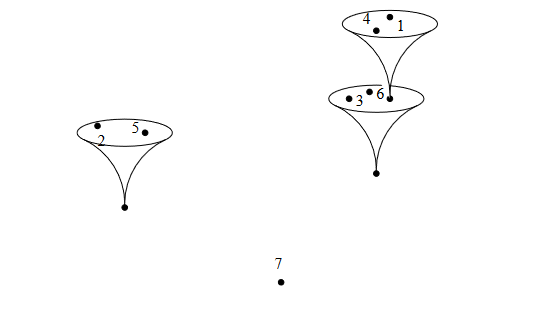
\includegraphics[width=0.8\textwidth]{img/sinha-fm-element}
    \caption{A point in $\Conf_M(6)$ associated to a tree with four internal nodes. }
\end{figure}    

\begin{definition}
    An $f$-tree is a rooted connected tree with labelled leaves and no bivalent internal vertices. The root is allowed to be bivalent (and also univalent).
    
    By defining a relation via edge contraction, one obtains a poset structure on the set of $f$-trees with $k$ leaves, denote this by $\Phi_k$.
\end{definition}
See figure~\ref{sinha-trees} for an example.

\begin{figure}[ht]
    \centering
    \begin{subfigure}[b]{0.45\textwidth}
        \centering
        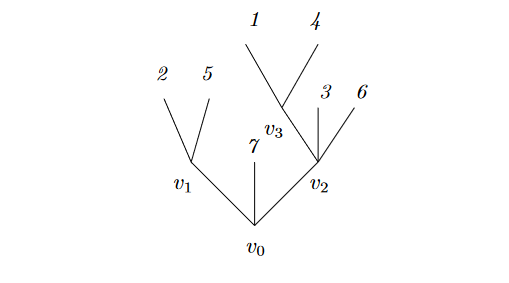
\includegraphics[width=\textwidth]{img/sinha-tree}
        \caption{An $f$-tree}
    \end{subfigure}
    \hfill
    \begin{subfigure}[b]{0.45\textwidth}
        \centering
        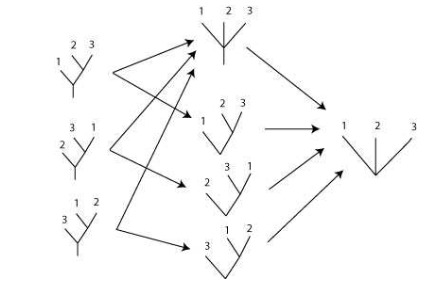
\includegraphics[width=\textwidth]{img/sinha-tree-poset}
        \caption{The poset $\Phi_3$ }
    \end{subfigure} 
    \caption{Example of $f$-trees. }\label{sinha-trees}
\end{figure}


\begin{theorem}
    There is a stratification on $\cConf_M(n)$ where each stratum $\cConf_M(T)$ corresponds to an $f$-tree $T$ and the poset of the stratification is $\Phi_n$. Similarly, for $\cConf_m(n)$, there is a stratification where each stratum $\cConf_m(T)$ corresponds to an $f$-tree $T$ where the root has degree at least $2$. 
\end{theorem}


\paragraph{Operad Structure on $\cConf_m(n)$} In the $M=\R^m$ case one may equip $\cConf_m(n)$ with an operad structure using the stratification explained earlier. 
\begin{theorem}
    The operad $\cConf_m$ is equivalent to the little $2$-disks operad $\mathcal D$.
\end{theorem}

To see this, we define a structure of an ``operad up to homotopy'' on $\Conf_n(m)$ (this is not standard terminology), in the sense that the associativity of composition does not hold on the nose, but there are canonical homotopies. There is then a zig-zag $\cConf_m \leftarrow \Conf_m \to \mathcal D_m$, where the first map preserves the operadic composition operations and is a homotopy equivalence on each level. The second map preserves the operadic composition operations up to homotopy and is also a homotopy equivalence on each level. This is enough to show that the homological operad structures agree, for an actual homotopy equivalence, one uses the Boardman-Vogt construction, which is a cofibrant resolution of topological operads.

To describe the operad structure ``up to homotopy'' on $\Conf_m$ in more detail, define a map $\Conf_m(n) \to \mathcal D_m(n)$ by drawing an outer disk around the barycenter of the configuration and drawing small disks around each point in the configuration (the radii should depend continuously on the configuration). Using this map and the projection to the center map $\mathcal D_m(n) \to \Conf_m(n)$, one may transfer the composition operations of $\mathcal D_m(n)$ to $\Conf_m(n)$. If multiple compositions in $\Conf_m$ are performed, the disks may differ in size, which leads to different configurations, but there is a homotopy comes from rescaling the circles. 

For the $m=2$ case one can alternatively apply a recognition principle by Fiedorowicz: The symmetric group acts freely on $\Conf_n(\R^2)$ and the quotient $\Conf_n(\R^2) / S_n = \UConf_n(\R^2)$ has $\pi_1(\UConf_n(\R^2)) = B_n$, the braid group of $n$ braids. The universal cover of $\Conf_n(\R^2)$ is contractible and has a braid operad structure with free action. Any two such operads with contractible total space and free group action are equivalent. Quotienting the equivalence by $PB_n = \ker(B_n \to S_n)$ we obtain an equivalence of the original operads. Then show that this also holds for $\cConf_n(\R^2)$.


\paragraph{Operadic module structure of $\Conf_M$} We build a fiberwise version of the configuration spaces $\cConf^M(n) = Fr_M\times_{SO(n)} \cConf_m(n)$, where $Fr_M$ is the oriented orthonormal frame bundle of some (irrelevant) metric on $M$. This is an operad in spaces over $M$. Then $\cConf_M$ is an operadic right module over $\cConf^M$. If $M$ is framed, then $\cConf_M$ is a module over the $\cConf(\R^D)$ operad.






\section{Graph Complex of Configuration Spaces}

\subsection{The case $M=\R^m$}

\paragraph{Homology} We first exhibit a homological complex construction; this is ad-hoc, not following any reference. Recall from earlier that the homology is given as an operad generated by a multiplication $\mu$ and a bracket operation $b$. To a rooted binary tree with labeled vertices one can assign an element of $H_*(\Conf_m(n))$ by putting $b$ at each of the inner vertices. To a collection of such rooted trees (a forest), one can assign an element of $H_*(\Conf_m(n))$ by multiplying the previous elements up. These elements generate the homology as a module. 

We now create an operad of chain complexes related to rooted trees $\mathcal{RT}$, by using the same generators $\mu$ and $b=b_2$ as before, but we add generators $b_k\in\mathcal{RT}(k)$, which corresponds to a corolla with $k$ incoming vertices. Compositions of the generators $b_k$ can be graphically depicted as rooted trees, now no longer binary. $\mu$ is still commutative and associative. I haven't figured out how the Poisson relation translates to the higher terms, thus the operad structure is somewhat unclear for forest-like elements. The differential is given by the dual of edge contraction modulo some symmetries, so that the differential of $b_3$ is the Jacobi element of $b_2$. There is an exact sequence $H_{k(m-1)-1}(\Conf_m(k), \partial\Conf_m(k)) \to H_{k(m-1)-2}(\partial\Conf_m(k)) \to H_{k(m-1)-2}(\Conf_m(k))$. The generator $b_k$ represents the fundamental class of $H_{k(m-1)-1}(\Conf_m(k), \partial\Conf_m(k))$.

\paragraph{Cohomology} We now outline the complex descibing the cohomology of $\Conf_m(n)$. For a detailed construction, see \cite[Chapter 6]{lambrechts2014formality}. Consider diagrams (graphs) $\Gamma$ with $n$ labeled ``exterior'' points and an arbitrary finite number of indistinguishable ``interior'' points. Define a graded vector space freely generated by these graphs, where the degree of a graph is 
\begin{align*}
    \deg \Gamma = \abs{E_\Gamma} \cdot (m-1) - \abs{I_\Gamma} \cdot m.
\end{align*} 
We omit some details here: to choose appropriate signs in the differential later, one has to induce orders on most of the data of the graphs and talk about loops, parallel edges etc. The differential is given by edge contraction for edges with at least one internal vertex. Admissible diagrams contain no loops, no double edges, no internal vertices of valence $\leq 2$ and each internal vertex is connected to some external vertex. 

The admissible diagrams form a graph complex $\coGraphs_m$ with differential given by edge contraction. They form a Hopf cooperad with multiplication given by union of graphs, identifying the external vertices by their labels, and cooperadic cocomposition is dual to the operad with operadic composition $\comp_i$ which inserts at the node $i$ a graph and sums over all choices of connecting the loose edges to $i$. 

\begin{theorem}
    The complex of admissible diagrams is quasi-isomorphic to the singular cochain complex of $\cConf$.
\end{theorem}

\paragraph{Graph Complex according to Idrissy \cite{idrissi2021real}} Assume $M$ is a simply connected compact manifold and $A$ a Poincaré duality model of $M$. The Lambrechts-Stanley model of $\Conf_m(r)$ is the chain complex 
\begin{align*}
    G_A(r) \defeq A^{r\otimes} \otimes S(\omega_{ij})_{1 \leq i\neq j\leq r} / I.
\end{align*}
where $I$ is generated by 
\begin{itemize}
    \item the relations $\omega_{ij}^2, \omega_{ji} = (-1)^m \omega_{ij}$, $\omega_{ij}\omega_{jk} + \omega_{jk}\omega_{ki} + \omega_{ki}\omega_{ij} = 0$ that appear in the presentation of the cohomology by Arnol'd.
    \item $p_i^*(a)\omega_{ij} = p_j^*\omega_{ij}$ for an $a\in A$ and $1\leq i\neq j \leq r$. 
\end{itemize}

Here, $p_{ij} \colon A\otimes A \to A^{\otimes r}$ is $p_{ij}^*(a\otimes b) = p_i^*(a)\cdot p_j^*(b)$ where $p_i^*\colon A\to A^{\otimes r}$
\begin{align*}
    p_i^*(a) \defeq 1\otimes \cdots \otimes 1\otimes a\otimes\cdots\otimes 1
\end{align*}
with the $a$ in the $i$-th position. 

The differential $d = d_A + d_{split}$ on $G_A(r)$ is the sum of the differential induced by that on $A$ and replacing an edge by the diagonal class of $A$
\begin{align*}
    d_{split}(\omega_{ij}) = p_{ij}^*(\Delta_A).
\end{align*}



\paragraph{Intuition} The following is not meant to be precisely true, but it still gives good intuition. Let $\Gamma$ be an admissible diagram with $\ell$ interior vertices and fix an order on the interior vertices. Consider the intersection $\bigcap \pi_{ij}^{-1}(c_{ij})\subset \cConf_m(n+l)$, where $c_{ij}$ are constants. This is a space with expected codimension $\abs{(E_\Gamma)}\cdot (m-1)$, we interpret it as a homology class in $H_*(\cConf_m(n+\ell), \partial\cConf_m(n+\ell))$. Map this along the projection $p_{n,\ell}\colon \cConf_m(n+\ell)/\partial\cConf_m(n+\ell) \to \cConf_m(n)/\partial\cConf_m(n)$ which forgets the last $\ell$ points, denote the resulting class by $a_\Gamma\in H_*(\cConf_m(n), \partial\cConf_m(n))$, now of expected codimension $\abs{(E_\Gamma)}\cdot (m-1) - \ell\cdot m$. The boundary of the space is given by edge contraction of $\Gamma$. Under Poincare duality, it corresponds to the form $\bigwedge \alpha_{ij}$ of degree $\abs{E_\Gamma}\cdot (m-1)$. 

For example, figure \ref{graph-complex-ex} shows how the Arnol'd identity $\alpha_{12}\alpha_{23} + \alpha_{23}\alpha_{31} + \alpha_{31}\alpha_{12} = 0$ in cohomology arises in this way: Interpret the diagram in (b) as the space of configurations of four points where the relative directions between the interior and the exterior point are fixed. The codimension one boundary of this is given by the configurations where the interior point is infinitesimally close to one of the three exterior points (and the relative directions are still fixed). Forgetting the interior point now yields three components as in (a).  

\begin{figure}[ht]
    \centering
    \begin{subfigure}[b]{0.65\textwidth}
        \centering
        \includesvg[width=\textwidth]{img/graph-complex-jacobi-2}
        \caption{The Arnol'd identity $\alpha_{12}\alpha_{23} + \alpha_{23}\alpha_{31} + \alpha_{31}\alpha_{12} = 0$}
    \end{subfigure}
    \hfill
    \begin{subfigure}[b]{0.3\textwidth}
        \centering
        \includesvg[width=\textwidth]{img/graph-complex-jacobi-1}
        \caption{A cochain whose boundary is the Arnol'd identity}
    \end{subfigure} 
    \caption{Arnol'd identity in the graph complex. }\label{graph-complex-ex}
\end{figure}

This intuition the definition of the boundary operator and the product structure. The operad structure is not immediately clear. 

Note that the projection $\cConf_m(n+\ell) \to \cConf_m(n)$ becomes an umkehr map in cohomology due to Poincare duality. Thus one can use fiber integration to represent this. The construction ``configuration space integral'' quasi-isomorphism $Graphs_m \to \Omega_{PA}(\cConf_m)$ essentially works as described above. The construction of the umkehr map is difficult, as the fiber is not a manifold, hence one uses PA forms here. 

\subsection{The case $M$ manifold}

Following \cite{campos2016model}. 

%\paragraph{Decorated Graphs} Let $H$ be a vector space and $S$ be a collection of graphs with vertex sets $V_G$ for $G\in S$. The vector space of decorated graphs is the space

%\begin{align*}
%    \bigoplus {G\in S} \Lambda(H_v \mid v\in V_G)
%\end{align*}

%where $\Lambda$ is the commutative algebra generated freely by the vector spaces and the $H_v$ are distinct copies of $H$ for each vertex $v$. Thus each vertex may be decorated with multiple elements of $H$ at each vertex, which are related tensorially. 

% \paragraph{Pre-dual graphs} Let $V$ be an $N$-dimensional graded vector space with a non-degenerate pairing of degree $-D$; $\langle\blank,\blank,\rangle\colon V\otimes V \to \R$ s.t. $\langle x, y\rangle = (-1)^{kl+d}\langle y, x\rangle$. The example to keep in mind is the cohomology of a connected $N$-manifold. We may require that the pairing is compatible with the multiplication or a differential. 

% Let $e_1, \dots, e_N$ be a basis of $V$. Denote by $\coGra_V(n)$ the free graded commutative algebra generated by symbols $s^{ij}$ of degree $D-1$ for $i,j \leq n$ and $e_1^j\dots e_N^j, j=1,\dots,n$, quotiented by $e^j_1 - 1$. Define a differential via 
% \begin{align*}
%     &de^j_\alpha = 0 \\
%     &ds^{ij} = \sum_{\alpha, \beta} g^{\alpha\beta}e^i_\alpha e^j_\beta
% \end{align*}
% where $g^{kl}$ is the inverse of the matrix describing the pairing on $V$ (so $\sum_{g^{\alpha, \beta}} e_\alpha e_\beta$ is the ``diagonal class'' i.e.\ the associated copairing). More abstractly, one can also present this without choosing a basis in $V$, by considering the graded commutative algebra generated by $n$ different copies of $V$ and the free symbols $s^{ij}$. A homogeneous element corresponds to a graph with $n$ vertices and decorations at each vertex with elements of $V$, see figure \ref{cw-graph-example}. 

If $M$ is a compact orientable manifold, denote by $\coGra_M(n) = \coGra_{H^*(M)}(n)$. If $M = \R^D$ and hence $V=k$ concentrated in degree $0$, then the above construction, omitting differentials, yields a graded vector space, which we denote $\coGra_D(n)$; this corresponds to undecorated differentials. 

$\coGra_D$ is a cooperad and $\coGra_M$ is a comodule of $\coGra_D$. 

\begin{figure}[ht]
    \centering
    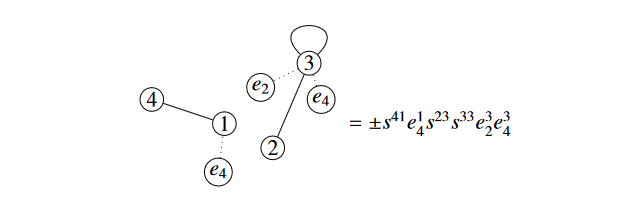
\includegraphics[width=0.8\textwidth]{img/campos-willacher-graph-dual-example.png}
    \caption{An example of a graph describing an element in $\coGra_V(4)$}\label{cw-graph-example}
\end{figure}

\paragraph{The dual graph complex $\coGraphs_M(n)$} As a vector space, it is spanned by $n$ labeled external vertices and an arbitrary finite number of internal vertices, decorated by (possibly multiple) cohomology classes of deg $\geq 1$, under the condition that there are no connected components without external vertices. There is a graded commutative algebra structure given by superposition of external vertices (i.e. disjoint union of graphs followed by identifying the external vertices with the same label). The differential splits as $\delta_{contr} + \delta_{cut} = \delta_{contr} + \Delta^* + \delta_{Z_M}$, where $\delta_{contr}$ contracts edges with at least one internal vertex and $\delta_{cut}$ splits edges with the copairing. This may produce ``forbidden'' graphs containing connected components without external vertices. This is the $\delta_{Z_M}$ part, which maps these components to a scalar via the function $Z_M$.

There is a similar construction for the $M=\R^D$ case for $\coGraphs_D(n)$, the difference is that all internal vertices of graphs are required to be at least trivalent (and no decorations are required). This has a cooperad structure which is induced by the dual of contracting a subgraph: for the coaction on a graph $\Gamma$ one sums over tuples $\Gamma', \Gamma_1, \dots, \Gamma_k)$ such that when each graph $\Gamma_i$ is inserted at the vertex $i$ of $\Gamma'$, one can reconnect the loose edges such that one obtains $\Gamma$.  

TODO: Image

\begin{theorem}
There is a quasi-isomorphism between $\coGraphs_D$ and $\Omega_{PA}(\cConf_D)$ (which is equivalent to $\mathcal A_{PL}(\cConf_D)$), which is compatible with the cooperad structures (in an appropriate sense).

There is an equivalence between $\coGraphs_M$ and $\mathcal A_{PL}(\cConf_M)$ which is compatible with the cooperadic comodule structure. 
\end{theorem}

\begin{figure}[ht]
    \centering
    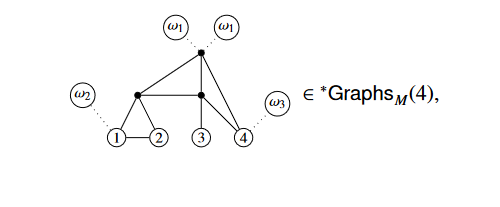
\includegraphics[width=0.5\textwidth]{img/cw-graphs-ast-example.png}
    \caption{An example element of $\coGraphs_V(4)$}\label{cw-graphs-ast-example.png}
\end{figure}    
\begin{figure}[ht]
    \centering
    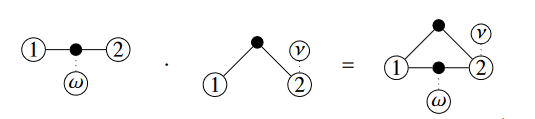
\includegraphics[width=0.7\textwidth]{img/cw-graphs-mult.png}
    \caption{An example element of $\coGraphs_V(4)$}\label{cw-graphs-mult}
\end{figure}



\nocite{*}
\bibliography{bibliography}

\end{document}






























\section{Loop Space}

Presentations of $S^1$ as a homotopy colimit usually induce presentations of the free loop space as as homotopy limit. 
\begin{align*}
S^1 &= \hocolim \{* \rightrightarrows *\} \\
\Lambda X &= \holim \{ X \rightrightarrows X\}
\end{align*}
Here the arrows are two copies of the identity map.

\begin{align*}
S^1 &= \hocolim \{* \coprod * \rightrightarrows * \} \\
\Lambda X &= \holim \{ X \rightrightarrows X \times X \} = X \times_{X\times X} X
\end{align*}
Here the arrows are two copies of the unique map resp.\ the diagonal map.

A computation of the first homotopy limit via the Bousfield-Kan approach / Reedy models leads to the following cosimplicial space

\begin{tikzcd}
    X \arrow[r, shift left=1]\arrow[r, shift right=1] & X \times X \rar[shift left = 2]\rar\rar[shift right=2] & X \times X \times X \rar[shift left=3]\rar[shift left=1]\rar[shift right=1]\rar[shift right=3] & X \times X \times X \times X \dots
\end{tikzcd}

The $i$-th boundary map $X^n\to X^{n+1}$ duplicates the $i$-th element into the $i$-th and ($i+1$)-th position modulo $n+1$. The degeneracy maps erase any except the first element.

The totalization $Tot(X_\bullet)$ of a cosimplicial space $X_\bullet$ is the space of natural transformations $Map(\Delta^*, X_\bullet)$, where $\Delta^*$ is the standard cosimplicial space. Its topology is the subspace topology from the inclusion into $\Prod_n X_n^{\Delta^n}$.

If $X_\bullet$ is the cosimplicial space associated to the loop space as above, then its totalization is indeed the loop space: one checks that the higher simplices are uniquely determined by the $1$-simplex through the degeneracy maps. 

Composing the cosimplicial object $X_\bullet$ with the singular chain complex functor yields a cosimplicial chain complex whose totalization is quasi-isomorphic to the coHochschild chain complex. Dually, applying the singular cochain functor yields a simplicial chain complex whose realization is quasi-isomorphic to the Hochschild chain complex. Hence we are interested in how totalization and the chain complex functors commute. 

The result that we are looking for is that taking homotopy limits/colimits of topological spaces resp.\ chain complexes commutes with the chain complex functors. The classical way to do this is via Quillen adjunction, but we would like to see this done via $\infty$-categories. Afterwards we just have to check how the homotopy limit of chain complexes is computed. 

Patras-Thomas give a morphism 
\begin{align*} 
    \phi\colon \realization{NC(X^K)}^* \to C^*(\totalization{X^K}),
\end{align*}
where $NC$ is the normalized complex and bars are realization of a simplicial chain complex resp.\ totalization of a cosimplicial space. They show that under certain assumptions on connectedness this yields an isomorphism of cohomology algebras. The map $\phi$ is defined as follows: let $\underline{Z}$ be a cosimplicial space, then 
\begin{align*}
    \phi_{p,s}\colon C^{p+s}(\underline Z[p]) \xrightarrow{e_p^*} C^{p+s}(\Delta^p \times \totalization{\underline Z}) \xrightarrow{\int_{\Delta^p}} C^s(\totalization{\underline{Z}})
\end{align*}
Note that $e_p$ composes to a morphism of cosimplicial spaces $\underline{\Delta} \times \totalization{\underline{Z}} \to \underline Z$. The dual map is
\begin{align*}
    C_{p+s}(\underline Z[p]) \xleftarrow{e_p} C_{p+s}(\Delta^p \times \totalization{\underline Z}) \xleftarrow{\times \Delta^p} C_s(\totalization{\underline{Z}})
\end{align*}
This can also be seen as a map
\begin{align*}
    \phi_p\colon C_*(\totalization{\underline{Z}}) \xrightarrow{[\Delta^p] \times} C_{*+p}(\Delta^p \times \totalization{\underline Z}) \to C_{*+p}(\underline{Z}[p])
\end{align*}
This gives a total map 
\begin{align*}
    \phi &\colon C_{*}(\totalization{\underline{Z}}) \to \Prod_{p} C_{*+p}(\Delta^p \times \totalization{\underline Z}) \to \Prod_{p} C_{*+p}(\underline Z[p]) \\
    \phi &\colon C_{*}(\totalization{\underline{Z}}) \to \totalization{ C_{*}(\underline{\Delta} \times \totalization{\underline Z})} \to \totalization{C_{*}(\underline Z)} \\
\end{align*}
Setting $\underline Z = X^{S^1_\bullet}$:
\begin{align*}
    C_*(\Lambda X) \to C_{*+p}(\Delta^p \times \Lambda X) \to C_{*+p}(X^{p+1})
\end{align*}
and one can check that the right map is indeed given by evaluation. 


\section{CoHochschild Construction and Base Points}

The usual cobar and coHochschild constructions are applied to $C \coloneqq C_*(X, x)$, the complex generated by singular simplicial maps with vertices mapped to a fixed $x\in X$. This seems sensible for the cobar construction, which models the based loop space, but for the free loop space, we would like to omit the choice of base point. 

Recall that the singular complex $C_*(X)$ is a coalgebra with two $C_0 \coloneqq C_0(X)$-coactions $\lambda \colon C\to C_0 \otimes C$ resp. $\rho\colon C\to C\otimes C_0$ from the left and the right, which extract the first resp. last last vertex of a singular simplex. Let $\tau\colon C_1 \otimes \dots \otimes C_k\to C_2 \otimes C_k \otimes C_1$ be the cyclic permutation map with the usual Koszul sign. There are $k$ pairs of parallel maps $C^{\otimes k} \to C \otimes C_0 \otimes C^{k-1}$ given by $(\rho \otimes id^{k-1})\tau^i$ resp. $(id\otimes \lambda\otimes id^{k-2}) \tau^i$. 
\begin{definition}
    The cyclic cotensor product $C^{\square k} \subset C^{\otimes k}$ is the collection of those elements such that each pair of coaction maps as defined above agrees. More generally, one can define a cyclic cotensor product of a tuple of bicoalgebras.
\end{definition}
This means that the sum of first vertices in the $i+1$-th factor agrees with the sum of last vertices in the $i$-th factor. 
Note that even in for $k=1$ this is generally a nontrivial condition and we have in particular defined $C^{\square 1} = C^\square\subset C$. 

This is not a complex using the differential on $C^{\otimes k}$, because the outer face maps $\partial_0$ and $\partial_k$ do not respect the imposed condition. One can obtain a complex by defining a differential which omits the outer face maps. 


\section{Spectra}
Let $Sp$ be the category of spectra. $Sp$ is closed monoidal with the smash product $\wedge$ and the sphere spectrum $\mathbb S$. There is a functor $\Sigma^\infty\colon Top_* \to Sp$ resp.  $\Sigma_+^\infty\colon Top \to Sp$ with an adjunction $\Sigma^\infty_+ \dashv \Omega^\infty$. The homology wrt a homology theory associated to a spectrum $E$ can be computed via 
\begin{align*}
    H_\bullet(X, E) &= X \wedge E  &&H_n(X, E) = \pi_n(X \wedge E) = [\Sigma^n \mathbb S, X\wedge E] \\
    H^\bullet(X, E) &= [X, E]  &&H^n(X, E) = \pi_n([X, E]) = [\Sigma^n \mathbb S\wedge X, E]
\end{align*}

\paragraph{Umkehr maps} Given an embedding of closed manifolds $P\subset N$ and a vector bundle $\xi$ on $N$, one can give an umkehr map $f_\xi^! \colon N^\xi \to P^{\nu + \xi}$ of Thom spectra, where $\nu$ is the normal bundle of $P$.
\end{document}
